\chapter{Planificación}
\label{chap:planificacionProyecto}
\lettrine{E}{n} este capítulo se propone una planificación del proyecto con el fin de organizar su estructura y exponer sus costes temporales y económicos aproximados necesarios para su realización.

\section{Tareas}
\underline{Tarea 1}. Analizar como está formada la infraestructura, que componentes hardware y software la componen y cual es la función de cada uno de ellos.\\

\underline{Tarea 2}. Analizar y seleccionar una herramienta de las disponibles en el mercado que se adapte a las necesidades del servicio que se quiere construir y a las características de la infraestructura.\\

\underline{Tarea 3}. Despliegue de la plataforma seleccionada sobre la infraestructura existente.\\

\underline{Tarea 4}. Configuración de los parámetros de la plataforma una vez desplegada.\\

\underline{Tarea 5}. Diseño de la integración de la nueva plataforma con el sistema de autenticación de la UDC.\\

\underline{Tarea 6}. Implementación y despliegue de la integración para la autenticación de usuarios con sus credenciales de la UDC.\\

\underline{Tarea 7}. Análisis del uso que harán los usuarios del servicio para establecer políticas sobre el uso de recursos.\\

\underline{Tarea 8}. Diseño de un sistema de facturación/valoración de los recursos del servicio en base a las políticas de uso establecidas.\\

\underline{Tarea 9}. Implementación y despliegue del sistema de facturación valoración diseñado.\\

\underline{Tarea 10}. Recopilación de la información necesaria para la realización de cada tarea. Esta tarea se realiza de forma continua a lo largo de todo el proyecto.\\

\underline{Tarea 11}. Redacción de la memoria del proyecto. Esta tarea se realiza de forma continua a lo largo de todo el proyecto.\\

La duración total del proyecto se estima en 165,25 horas repartidas durante 42 días teniendo en cuenta que el estudiante trabaja durante 4 horas diarias. El coste mostrado se refiere al coste correspondiente al estudiante si trabaja por 15 €/hora[\ref{fig:estadisticasproyecto}]. 

\begin{figure}[h!]
  \centering
  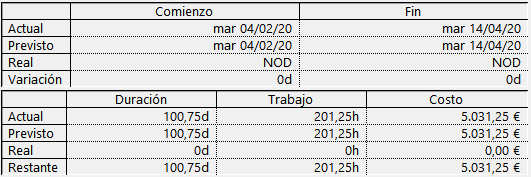
\includegraphics[width=1\textwidth]{imaxes/extras/estadisticasProyecto.png}
  \caption{Estadísticas sobre la planificación del proyecto.}
  \label{fig:estadisticasproyecto}
\end{figure}
\begin{figure}[h!]
  \centering
  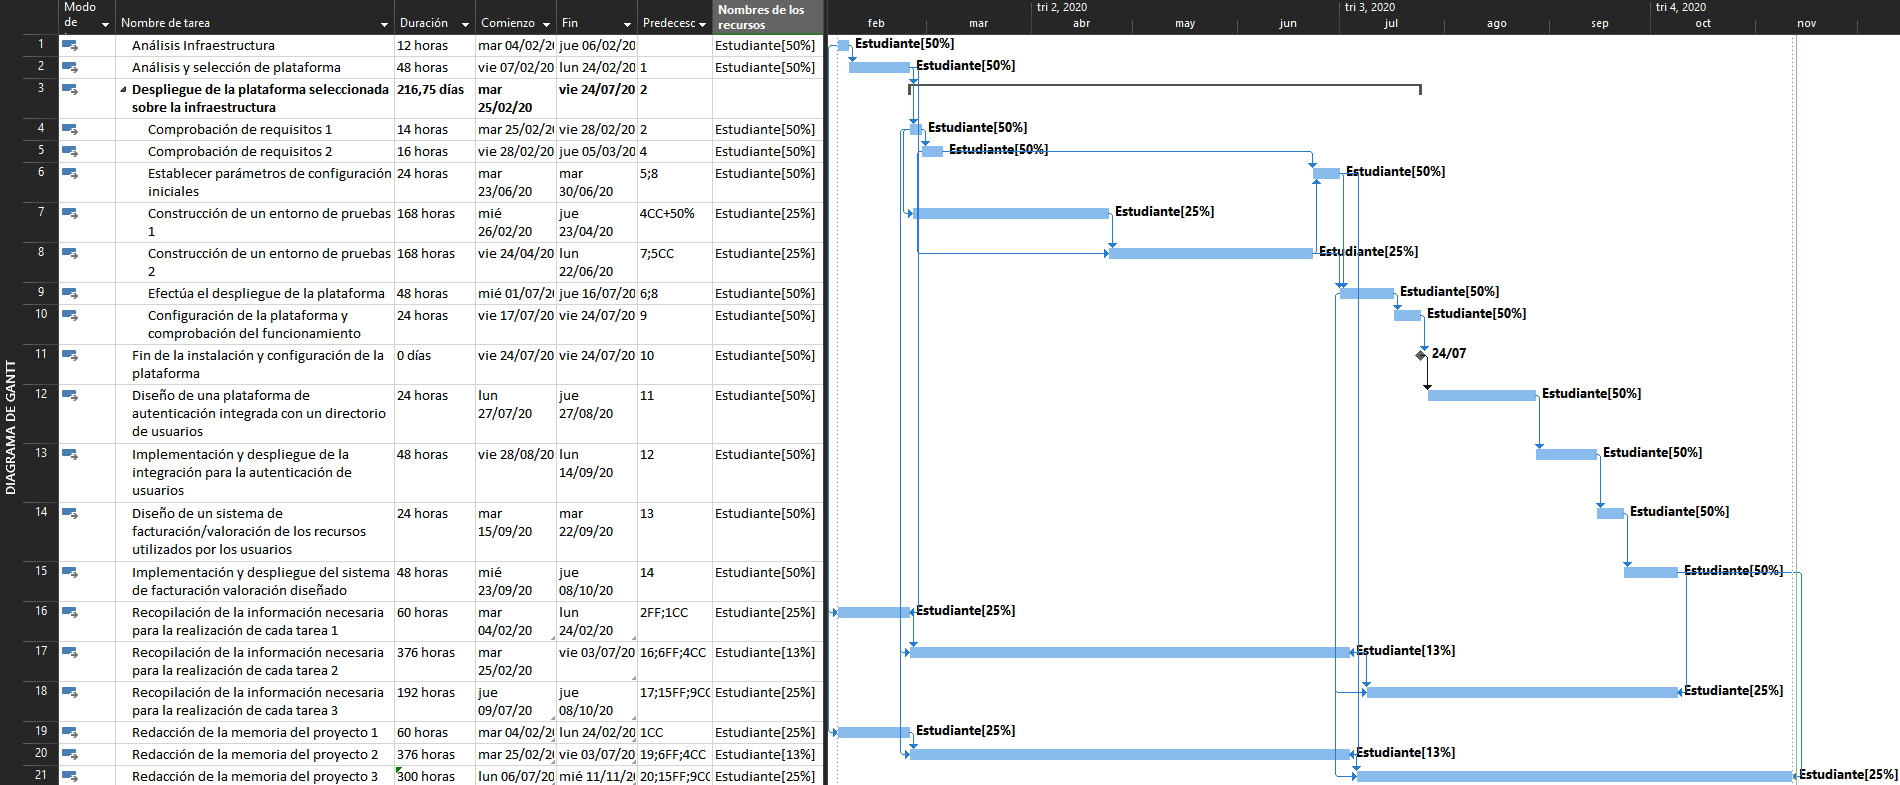
\includegraphics[width=1\textwidth]{imaxes/extras/diagramaGranttt.png}
  \caption{Diagrama de Grantt sobre la planificación del proyecto.}
  \label{fig:tareasproyecto}
\end{figure}

\section{Costes}